\label{appendix:system_identification}
\section{System Identification}

\subsection{Data Collection}
The Pixhawk autopilot was used to capture roll and pitch rates $(\dot{p},\dot{q})$ for the test vehicle as well as the pilot's command inputs.  These outputs and inputs were the essential building blocks for creating pitch rate and roll rate models for the test vehicle.  The autopilot is capable of logging data at 50-400 Hz and therefore is a discrete time domain signal.  This data should ultimately be manipulated into the s-domain.  The mathematics for this procedure are well defined, and numerous tools can be used to simplify this process.  

It is crucial to ensure there is sufficient frequency content in the data recorded.  Exciting multiple frequencies in the time domain ensures the regression techniques have an adequate sample space to search for polynomial coefficients.  Exciting adequate frequency inputs is analogous to only sampling at one independent variable and expecting to get a regression fit from a non-changing dependent variable.  

To ensure sufficient frequency content was obtained from the aircraft, a linear chirp was chosen and implemented into the Pixhawk source code as follows:

\begin{equation}
x(t)=sin\left[\phi_0+2\pi\left(f_0t+\frac{k}{2}t^2\right)\right]
\end{equation}

where:
\begin{itemize}
 \item[] $\phi_0$ is the initial phase of the chirp at t=0 (nominally zero degrees)
 \item[] $f_0$ is the initial frequency at t=0
 \item[] $k$ is the chirp rate
 \item[] $t$  is time in seconds
\end{itemize}

An example of this formulation can be seen below:

\begin{figure}[!h]
 \centering
  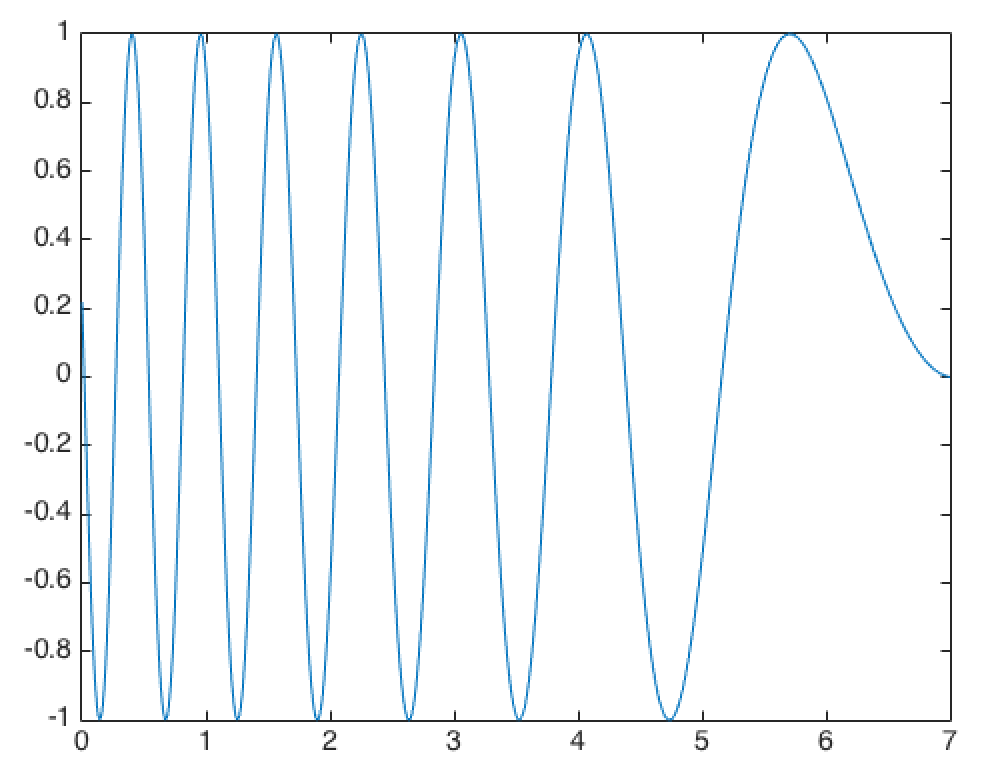
\includegraphics[width=0.50\textwidth]{chirp.png}
  \caption{Reverse Linear Chirp Example}
  \label{fig:chirp}
\end{figure}

\subsection{z-Domain to s-Domain}
The logged input and output data in discrete form requires shaping to convert cleanly into an s-domain representation.  The first step is ensuring that the data is of constant sampling rate.  In other words, the time between samples is uniform from sample to sample.  The data provided from the Pixhawk autopilot does not have a uniform sampling rate.  The sample rate is a user-defined rate (50-400Hz) but has a slight amount of jitter $(\pm 0.1\%)$.  \ac{PCHIP} interpolation was used to interpolate the data into a uniform sampling rate.

After the data is shaped correctly with a uniform sample rate, the discrete data is transformed into a continuous approximation using a \ac{ZOH} technique.  Taking the Laplace transform of the continuous input/output data will convert it into the s-domain, and finally, a non-linear least squares minimization algorithm can be run to find the polynomial coefficients which best fit the data.

The order of the regression (number of polynomials to estimate) is at the discretion of the engineer and their intuition of system's physical representation.  Higher order models will better fit the data, but in most cases tend to overfit the data if they cannot be justified by physical principles.  Most aircraft models assume that the system is \ac{LTI} and second order.  These fundamental aerodynamics models divide the modeling into longitudinal and lateral dynamics.  Each axis of the aircraft is assigned two, second order responses.  Pitch, for example, has a second order response in the pitch damping mode (also known as the short period) and also has a second order response in the transition of kinetic energy to potential energy (also known as the long-period or phugoid).  This would imply that the collected body rate data $(\dot{p},\dot{q})$ collected by the autopilot should be modeled as first order systems because body rate is the first derivative of attitude.  Assuming a first order system for the collected data in this experiment keeps the originally derived physical meaning but may be insufficient upon critical analysis.  Both first order and second order model were estimated for comparison sake.

Results were collected from two flight test events.  The first flight test was data collected prior to implementing the chirp, and the pilot attempted to increase frequency of the input signal manually.  The second set of data collected was via the reverse linear chirp method previously described.  

The manually piloted acquired data was expected not to have as adequate of frequency content in the signal but still provided adequate results for modeling the aircraft.

\begin{figure}[!h]
 \centering
  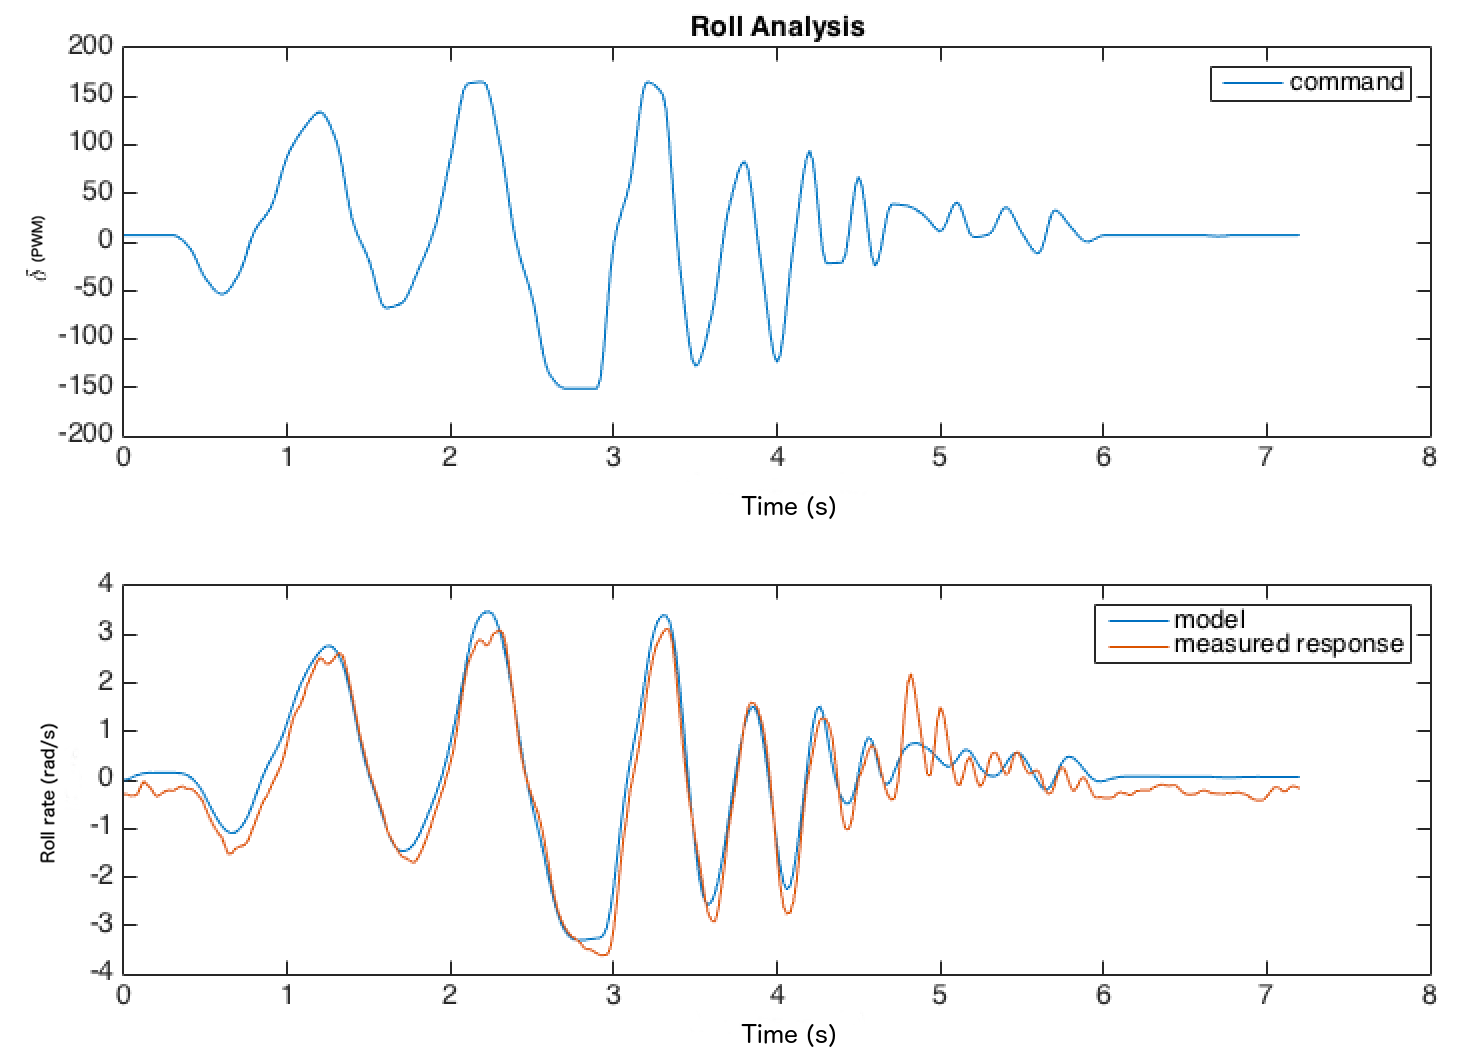
\includegraphics[width=0.75\textwidth]{model_response.png}
  \caption{Roll Model Regression with Manual Inputs}
  \label{fig:roll_model}
\end{figure}

The above result demonstrates the utility of this technique even with poorly structured data from manual pilot inputs.  It can be seen that the second order model starts to misrepresent the data at higher frequencies.  The lower frequency validity of this model showed potential and most of the high-frequency response may able to be neglected upon further review.  The following figure with the chirp results highlights the actual issue with the high-frequency modeling issues.

\begin{figure}[!h]
 \centering
  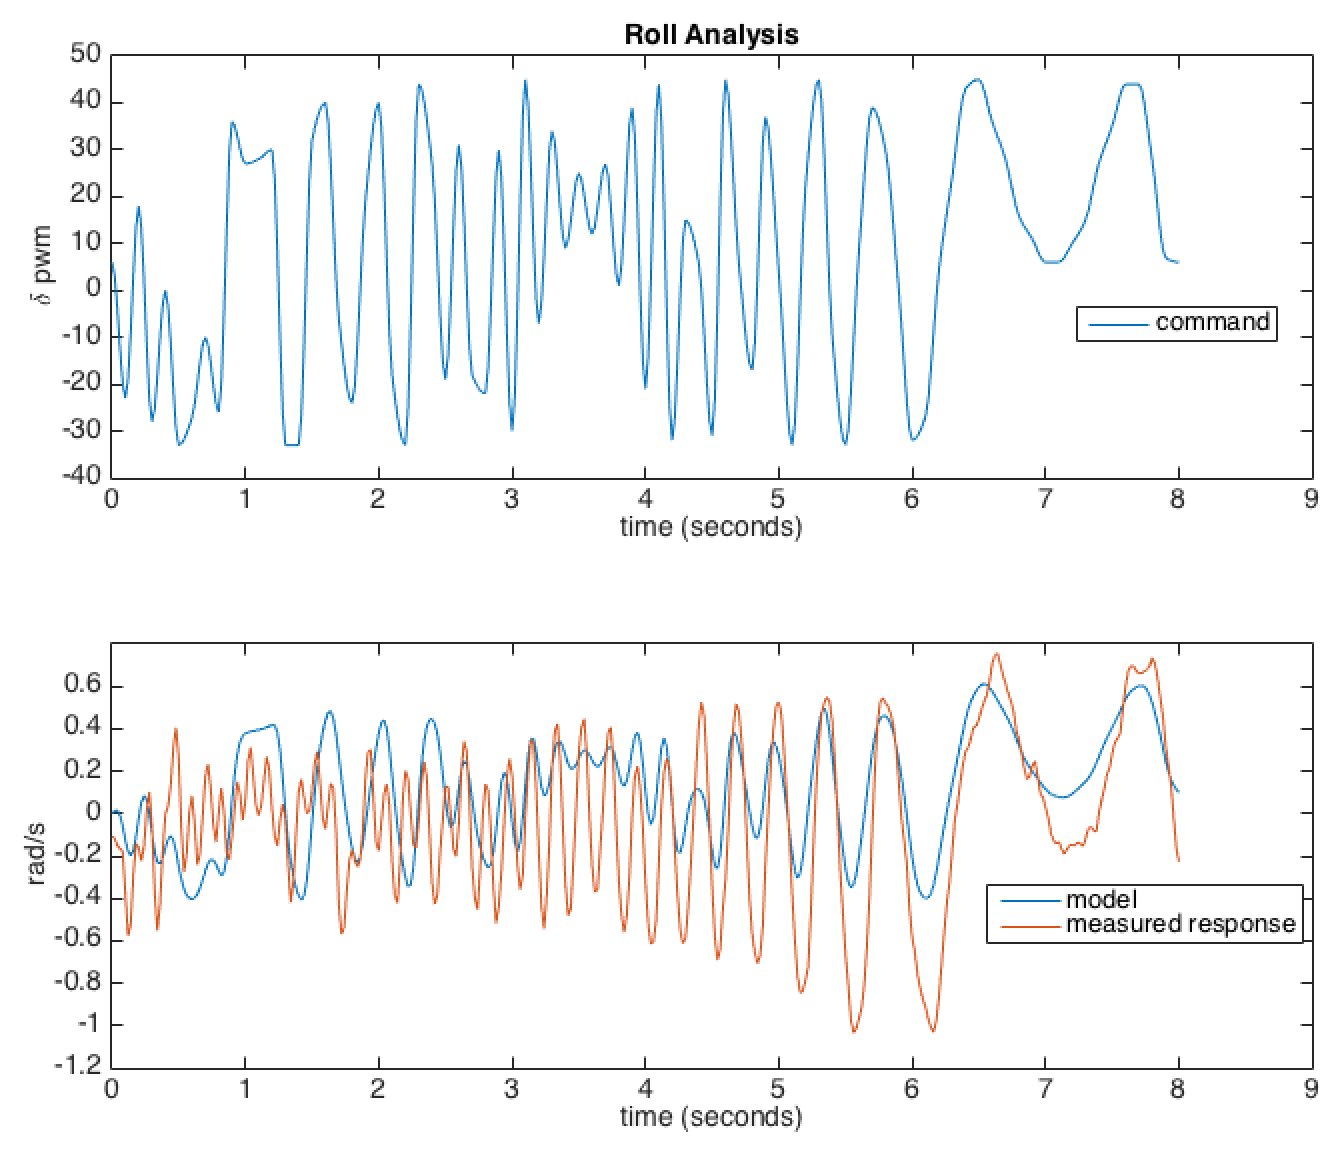
\includegraphics[width=0.75\textwidth]{chirp_response.png}
  \caption{Roll Model Regression with Reverse Linear Chirp}
  \label{fig:chirp_model}
\end{figure}

The reverse linear chirp, starting at high frequency and chirping down, clearly illustrates that this regression method has an underlying problem that was not evidently clear in the previous example.  In the chirp analysis, it is clear that the high-frequency modeling is in error.  After reviewing this result, it was clear that the sampling rate of the input channel was aliased.  The chirp response was physically observed on pre-flight, in actual flight, and in the actual body rate of the aircraft.  However, the aliased input channel was arbitrarily biasing the regression result.  The data was logged at 50 Hz with the assumption that 50 Hz was ten times higher than the expected natural frequency of the aircraft and at least five times higher than the Nyquist criterion.  The Nyquist criterion is the theoretical minimum frequency $(2f_0)$ to sample a signal and recover a given frequency.  The autopilot is capable of logging data at 400Hz, but in this case, the servo output loop is still at 50Hz due to it being the hardware bandwidth limit of standard \ac{RC} servos.  Some high-performance servos are capable of higher input frequencies, but this still wouldn't solve the specific issue found when running this analysis.  The peculiar aliasing issue is hardware specific to the Pixhawk 1 autopilot in how the main CPU sends servo commands to the auxiliary I/O  CPU.  The most recent version of firmware at the time of this test improperly logs the \ac{PWM} through an aliased prone signal path.  The main and I/O CPU both run at 50Hz with some appreciable clock drift.  This generates a noticeable beat frequency and delay when the actual values in registry are saved for \ac{PWM} values are sent back round trip to the main CPU.  The implication of logging the \ac{PWM} values at the very end of the digital transmission line seems valuable in principle because the values being logged are the undeniable values being sent to the actuators.  However, the cost of logging these values in this manner on the Pixhawk architecture incurs significant aliasing at almost all frequencies.  Logging the commanded \ac{PWM} values prior to being sent to I/O CPU solved the aliasing discrepancy and produced very frequency rich models.

The manually piloted acquired data provided viable data source for the models even though it is a very simplistic approach.  There were two separate manual tests run on the same aircraft on the same flight, and the following are the results using this regression technique to model a second order system.

\begin{equation}
H(s)=\frac{10.39}{s^2+31.26s+504.9}\
\end{equation}

and

\begin{equation}
H(s)=\frac{10.61}{s^2+29.77s+498.7}\
\end{equation}

Converting to standard form as described in equation~\ref{eq:second_order_model}:

\begin{equation}
H(s)=\frac{0.0206*22.47^2}{s^2+2*0.69*22.47s+22.47^2}\
\end{equation}

and

\begin{equation}
H(s)=\frac{0.0213*22.33^2}{s^2+2*0.67*22.33s+22.33^2}\
\end{equation}

It is important to note that this system identification technique run on separate sets of data has produced two models with very similar values for $\omega_n$ and $\zeta$.

This produces the average values of:

$\omega_n=22.4 rad/s$ \newline
$k = 0.0209$ \newline
$\zeta=0.681$ \newline

With the aliasing removed from the chirped input command signals as previously described, the model is drastically improved and produces the following results:

\begin{equation}
H(s)=\frac{4.409}{s^2+27.11s+430.6}\
\end{equation}

and

\begin{equation}
H(s)=\frac{3.295}{s^2+18.82s+2.96.5}\
\end{equation}

Converting to standard form as described in equation~\ref{eq:second_order_model}:

\begin{equation}
H(s)=\frac{0.0102*20.75^2}{s^2+2*0.65*20.75s+20.75^2}\
\end{equation}

and

\begin{equation}
H(s)=\frac{0.0111*17.21^2}{s^2+2*0.54*17.21s+17.21^2}\
\end{equation}

\begin{figure}[!h]
 \centering
  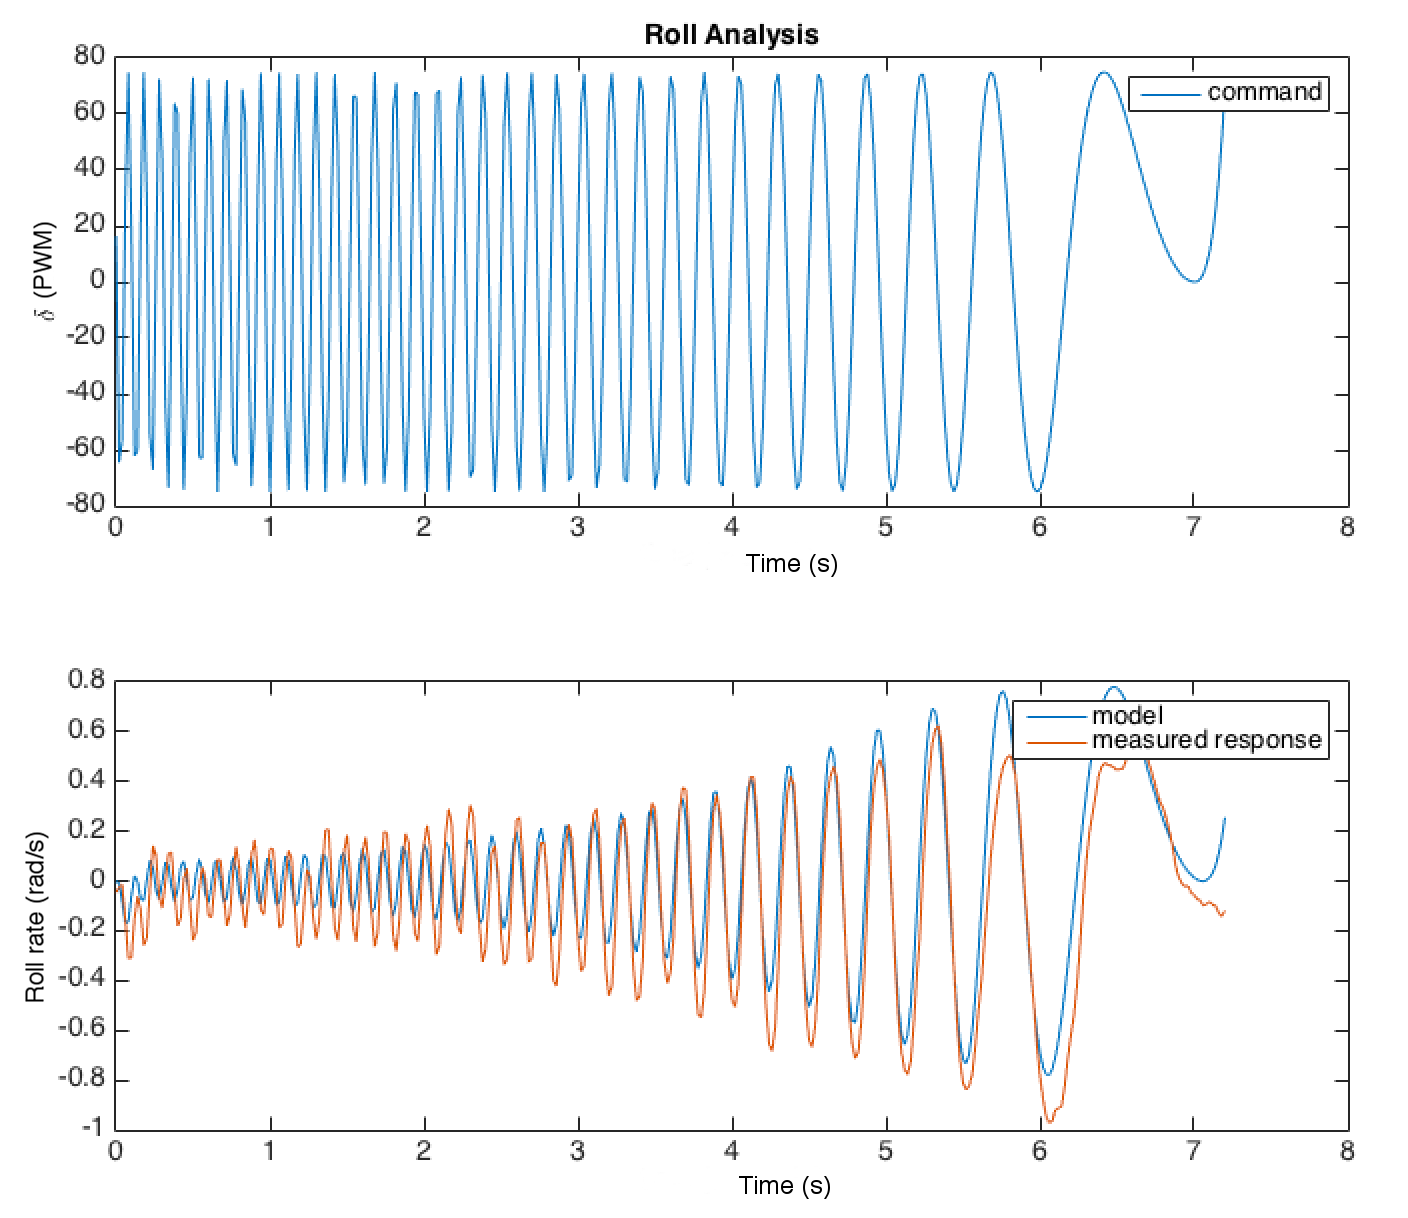
\includegraphics[width=0.75\textwidth]{reverse_chirp_roll.png}
  \caption{Non-Aliased Reverse Chirp model example}
  \label{fig:reverse_chirp_model}
\end{figure}

This produces the average values of:

$\omega_n=18.98 rad/s$ \newline
$k = 0.010$ \newline
$\zeta=0.598$ \newline

In the author's experience, these values are reasonable values for this size and weight of airframe.  This regression technique has shown potential to create realistic models from actual flight test data.  The data must be properly shaped.  The chirp method has the potential to increase the fidelity of the high-frequency response of the aircraft if the aliasing issue can be resolved on the command input channel.